\chapter*{Variabel Spyder}

\begin{enumerate}
   

\item buka spyder dan ketikan kode seperti berikut
	\begin{figure} [h]
	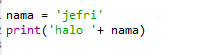
\includegraphics[width=10cm]{section/sp/sp5.png}
	\centering
	\end{figure}
	
	
\item pada kode berikut "jefri" merupakan value dan "nama" merupakan variabel
	\begin{figure} [h]
	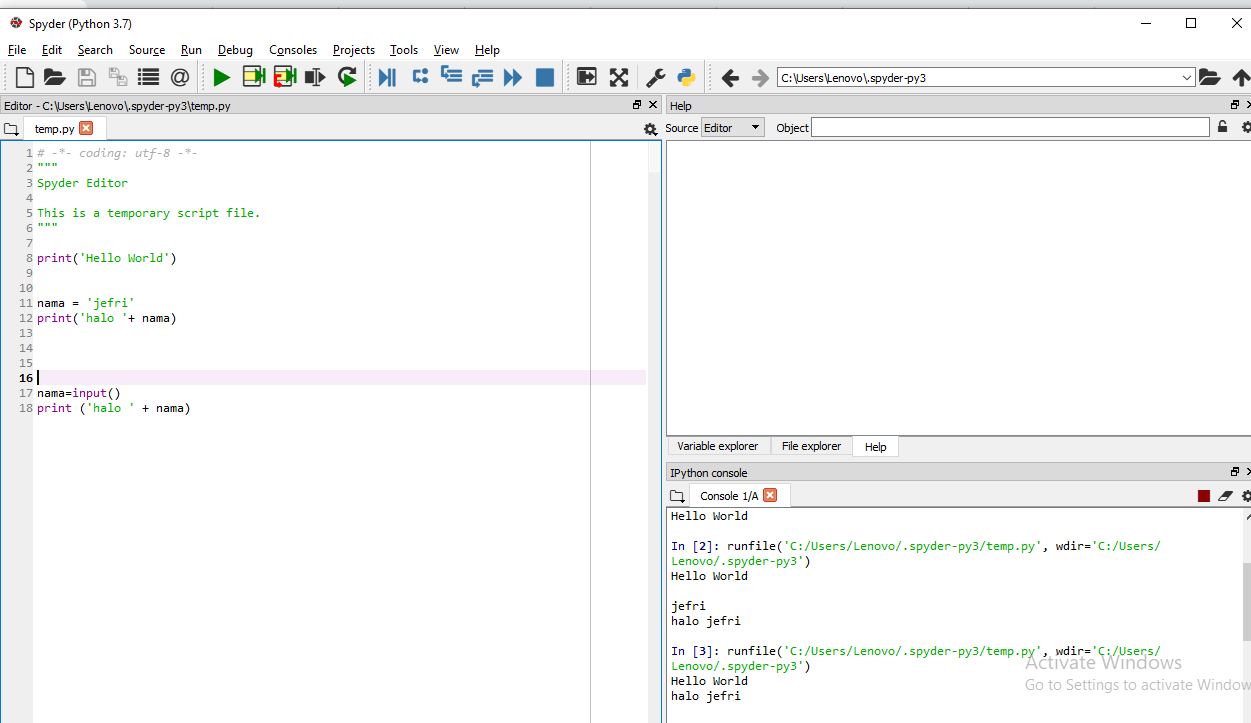
\includegraphics[width=12cm]{section/sp/sp6.png}
	\centering
	\end{figure}
	
 \item maka akan tercetak 
 \begin{figure} [h]
	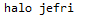
\includegraphics[width=6cm]{section/sp/sp7.png}
	\centering
	\end{figure}
 
	
	\end{enumerate}